		% options:
% thesis=B bachelor's thesis
% thesis=M master's thesis
% czech thesis in Czech language
% english thesis in English language
% hidelinks remove colour boxes around hyperlinks

\documentclass[thesis=M,english]{FITthesis}[2012/10/20]

% \usepackage[utf8]{inputenc} % LaTeX source encoded as UTF-8
% \usepackage[latin2]{inputenc} % LaTeX source encoded as ISO-8859-2
% \usepackage[cp1250]{inputenc} % LaTeX source encoded as Windows-1250

\usepackage{graphicx} %graphics files inclusion
% \usepackage{subfig} %subfigures
\usepackage{amsmath, kbordermatrix, amssymb} %advanced maths
\usepackage{amsthm} %theorems and lemmas
% \usepackage{amssymb} %additional math symbols
\usepackage[linesnumbered,lined,boxed]{algorithm2e}
\usepackage{enumitem}
\usepackage{dirtree} %directory tree visualisation
\PassOptionsToPackage{hyphens}{url}\usepackage{hyperref}
% % list of acronyms
% \usepackage[acronym,nonumberlist,toc,numberedsection=autolabel]{glossaries}
% \iflanguage{czech}{\renewcommand*{\acronymname}{Seznam pou{\v z}it{\' y}ch zkratek}}{}
% \makeglossaries

% % % % % % % % % % % % % % % % % % % % % % % % % % % % % % 
% EDIT THIS
% % % % % % % % % % % % % % % % % % % % % % % % % % % % % % 

\department{Department of Theoretical Computer Science}
\title{Meeting Scheduler}
\authorGN{Luk{\' a}{\v s}} %author's given name/names
\authorFN{Koc} %author's surname
\author{Luk{\' a}{\v s} Koc} %author's name without academic degrees
\authorWithDegrees{Bc. Luk{\' a}{\v s} Koc} %author's name with academic degrees
\supervisor{Ing. Jan Baier}
\acknowledgements{THANKS (remove entirely in case you do not with to thank anyone)}

\abstractEN{Summarize the contents and contribution of your work in a few sentences in English language.}

\abstractCS{V n{\v e}kolika v{\v e}t{\' a}ch shr{\v n}te obsah a p{\v r}{\' i}nos t{\' e}to pr{\' a}ce v {\v c}esk{\' e}m jazyce.}

\placeForDeclarationOfAuthenticity{Prague}
\keywordsCS{Replace with comma-separated list of keywords in Czech.}
\keywordsEN{Replace with comma-separated list of keywords in English.}
\declarationOfAuthenticityOption{1} %select as appropriate, according to the desired license (integer 1-6)

% \website{http://site.example/thesis} %optional thesis URL

%%%%%% Theorem package def
\newtheorem{theorem}{Theorem}
\newtheorem{lemma}{Lemma}
\renewcommand{\qedsymbol}{$\heartsuit$}
%%%%%% Theorem package def

%%%%%% Math def
\DeclareMathOperator{\atantwo}{atan2}
%%%%%% Math def

\begin{document}

% \newacronym{CVUT}{{\v C}VUT}{{\v C}esk{\' e} vysok{\' e} u{\v c}en{\' i} technick{\' e} v Praze}
% \newacronym{FIT}{FIT}{Fakulta informa{\v c}n{\' i}ch technologi{\' i}}

\setsecnumdepth{part}
\chapter{Introduction}

\section{Motivation}
The 21st century is often labelled as the century of data. Usage and gathering the data influence our lives on daily basis. Business, industry, fashion, society or transportation is transforming under the amount of data gathered and evaluated. 

Alongside the growing of the amount of data collected, borders with European countries are loosening and it is possible for people to travel within Europe in order to discover new cultures or to find a job in the country of their interest. Most of the time it is an unknown location. Finding meeting point with the colleagues or friends, which might not know the location as well, might turn into difficult task.

Applying the knowledge of graph theory, geography and computer science, the goal of the thesis is to create application finding ideal meeting place for a group of people, saving time for everyone involved.
Nowadays computers with multiprocessors or graphic cards are affordable for everyone, meaning paralellization of the computation is significant for every sophisticated application. Knowing that, the application should be designed to utilize possibilities of paralellization.

\section{Geographic information system}
Geographic information systems (GIS) are solving problems which are based on geospatial information. To achieve the goal special tools are being used such as visualization software, remote sensing and geography tools. Remote sensing tools gain information on specific objects or areas from a distance. Geography tools help to observe and research the environmental changes of the earth and its resources, its evolution of society and species. Visualization software, then, displays gathered data as 2D or 3D images \cite{Chen10}.

With a drastic change of modern technologies and enormous amount of data a new science was born---geographic information science---which is focusing on geographic concepts, applications and systems. The new science opens doors to new problems and issues at a global scale, not easily imaginable a few years ago. 

This thesis uses knowledge gathered through the course of time in geographic information science to map graph theory problems on real life data. The developed application belongs to the software category GIS software. 


\section{Problem description}

\subsection{Directed graph}
A directed simple \textit{graph} $G$ is a pair $(V, E)$, where $V$ is a finite set of \textit{vertices} and $E \subseteq V \times V$ are the $edges$ of a graph $G$. The number of vertices $|V|$ is denoted by $N$ and the number of edges $|E|$ is denoted by $m$ throughout this thesis, . A $path$ in $G$ is a sequence of vertices $v_1, v_2 \dots ,v_k$ such that $(v_i,v_{i+1}) \in E$ for all $1 \leq i < k$. A path with $v_1 = v_k$ is called a $cycle$. A graph (without multiple edges) can have up to $n^2$ edges. 

% We call a graph \textit{sparse}, if $m \in O(n)$. We assume that we are given a layout $L: V \to R^2$ of the graph in the Euclidean plane. For ease of notation, we will identify a node $v \in V$ with its location $L(v) \in R^2$ in the plane.

\subsection{Shortest path problem}
\label{sec:SPP}
Let $G = (V, E)$ be a directed graph whose edges are weighted by the function $f: E \to \mathbb{R}$. 
The length of a path is the sum of the weights of its edges. In this sense the weights can be reinterpreted as the edge lengths. A cycle whose edges sum to a negative value is \textit{negative cycle}.  

The shortest-path problem consists of finding a path of minimum length from a given source $s \in V$ to a given target $t \in V$.
Note that the problem is only well defined for all pairs, if $G$ does not contain negative cycles.
Since our problem is based on real values (distance between two points), negative weights and cycles do not occur in the rest of the thesis.
If there were negative weights, it is possible, using Johnson's algorithm \cite{Johnson77}, to convert the original weighting function $f: A \to \mathbb{R}$ to non-negative function $ f': A \to \mathbb{R}^+_0$ in time $O(n_m + n^2 \log n)$, which results in the same shortest paths.

\section{Organisation of the Thesis}
The thesis is structured as follows: First, the Chapter \ref{ch:DA} describes the desired attributes of the data and finding possible data sources. The chapter then further explains how the data can be stored and processed in order to reduce the number of unnecessary nodes. 

The next Chapter \ref{ch:DOTA} focuses on the overall design of the application, beginning with the algorithms solving the SSSP problem. The main algorithm used for our application is Dijkstra algorithm. In order to increase the computation time, the possible paralellization of Dijkstra algorithm is further explained. The application also requires basic user interface.

The Chapter \ref{ch:Realisation} describes the specific implementation of the application. More specifically how the application is implemented within server and client part, which frameworks were used and additional commentary of the code. 

The results of the application are concluded in Chapter \ref{ch:Results}, where we compare the results based on the accuracy and time comparison between parallel and single threaded implementation.
\setsecnumdepth{all}


\chapter{Data Analysis}
\label{ch:DA}

\section{Data fitness}
\label{S1: Good data}
As stated in Koc 2014 \cite{Koc14}, proficient functioning of the application requires a fitting data source. The application needs to work with reliable and (preferably) daily updated data. The area of coverage should not be limiting the application, so that a high number of users would find it convenient. The data format should be unified in order to make manipulation and management effective. Choosing the correct data format also enables the application to combine different data sources.

To sum up the data are required to follow certain criteria:
\begin{itemize}
	\item up-to-date
	\item verified
	\item human and computer readable
	\item easy-to-use and unified format
	\item freely available
	\item maintained, reliable
\end{itemize}



\section{Possible sources}

While searching for data, it was focused on sources providing free data of Europe, which is also available to the public. Further subsections describe sources which matched the criteria mentioned in section \ref{S1: Good data}.

%\subsection{Global map data}
%Global map data provided and managed by International Steering Commitee for Global Mapping.
%TODO
 
\subsection{EuroGeographics}
EuroGeographics is the membership association consisted of 60 organizations and 46 countries. It was created in year 2002, when the Comit{\' e}e Europ{\' e}en des Responsables de la Cartographie Officielle (CERCO) and the Multi-purpose European Ground Related Information Network (MEGRIN) merged together. Its goal is to gather and collect spatial and infrastructural data of Europe \cite{Euro16}. 

EuroGeographics association provides the following products: EuroBoundaryMap, EuroGlobalMap, EuroRegionalMap and EuroDEM.
EuroBoundary map mostly covers borders and administrative informations, EuroDEM map is commonly used for environmental change research or hydrologic modelling.
EuroGlobalMap and EuroRegionalMap consists of many datasets: the administrative boundaries, the water network, the transport network etc. 
In order to download the data it is required to fill up the registration form.

EuroGeographics provides data in following formats

\begin{itemize}
\item Geodatabase
\item Shapefile
\end{itemize}

EuroGeographics yield reliable source of data required by our application. Shapefile format can contain geographical data providing an option of additional attributes for the data. However, the registration form which needs to be filled almost every time in order to download the dataset makes the data processing cumbersome.

\subsection{OpenStreetMaps}
\label{subsec:DA_OSM}
OpenStreetMaps (OSM) is a project officially supported by the OSM Foundation.
OSM was created to build and provide open\footnote{Open data means for any purpose as long as the OSM and it's contributors are credited.} geographical data available to everyone.  

The OMS project was inspired by Wikipedia and is working exactly the same: Users are the ones contributing with their maps, gps measurements, aerial photographs etc. Since OSM creation in 2004, its community has significantly increased and the data are being updated daily.
OSM provides data in their .osm format, which follows XML rules.

In course of time a lot of projects were created which work with OSM maps.
Thanks to the team Mapzen and their Metro Extract project it is possible to download any major city data in additional two GIS data formats:
\begin{itemize}
\item Geojson
\item Shapefile
\end{itemize}

OSM data are regularly maintained by the community. Documentation to the data is well written, so that any discrepancy within the dataset can be easily resolved. The OSM format requires additional parsing in order operate with the data since it is not official GIS format, but projects as Mapzen provides additional format variety to choose from.

\subsection{EEA}
The European environmental agency (EEA) is an agency of European Union providing information about the environment for the public. According to their official site \cite{EEA16} it currently consists of 33 member countries.

EEA offers various different datasets, maps and graphs about national designated areas, ecosystem types of Europe, water state and quality, national communications etc. 

Depending on the type, these data are provided in the following formats:
\begin{itemize}
\item Excell table
\item CSV
\item Shapefile
\end{itemize} 

Most of the datasets are displayed in interactive maps available on the \href{http://www.eea.europa.eu/data-and-maps}{EEA website}.

After further investigation of the datasets provided by EEA, it seems they are not being updated regularly. In addition, most of the data sets are results of ecological studies or environmental researches (e.g. monitoring $CO_{2}$ or energy consumption).

\subsection{European Observation Network for Territorial Development and Cohesion}
The European Observation Network for Territorial Development and Cohesion (ESPON) 2013 Programme is mainly financed from European Regional Development Fund (ERDF) and its main goal is:

\textit{"Support policy development in relation to the aim of territorial cohesion and a harmonious development of the European territory \ldots "} \cite{ESPON13}

Data are available as soon as users register and accept the Terms \& Conditions. EPSON 2013 data are handled according to ISO 19115 scheme in two formats:

\begin{itemize}
\item XML
\item Excel file
\end{itemize}

Unfortunately, the data provided by ESPON are having a same disadvantage as data provided by EEA in previous section: maintainability. Our application require updated data sets in order to accurately compute the optimal meeting place. Investigating the ESPON page further, the ESPON project was separated into two phases, first phase starting in July 2008 -- February 2011 followed by second phase having a lifetime in span of February 2011 -- December 2014. 

As a data source the OpenStreetMaps were chosen since the data provided are regularly maintained by the community. In addition, the whole documentation in for of the wikipage contains all necessary information to learn the user how to fast start working with the data. As a format was chosen a Shapefile format, allowing the application to work with additional attributes if necessary (e.g. street names, type of road etc.).

\section{Format}
Geographical data exist in various formats depending on type and usage of the data. Data representing the elevation of mountains are better stored in different format whereas data representing the location of points of interest. 
Most of the existing formats typically fall into two main categories: vector format or raster format. 

% According to Esri's GIS dictionary %TODO cite
Both offer two different ways how to represent spatial data. However, the differences between vector and raster data types are equivalent to those in the graphic design world. The picture \ref{pic:RasterVector}, which graphically explains how these two types process given data, serves for a better understanding.
%http://i.stack.imgur.com/Y84dG.png

\begin{figure}[h]
\centering
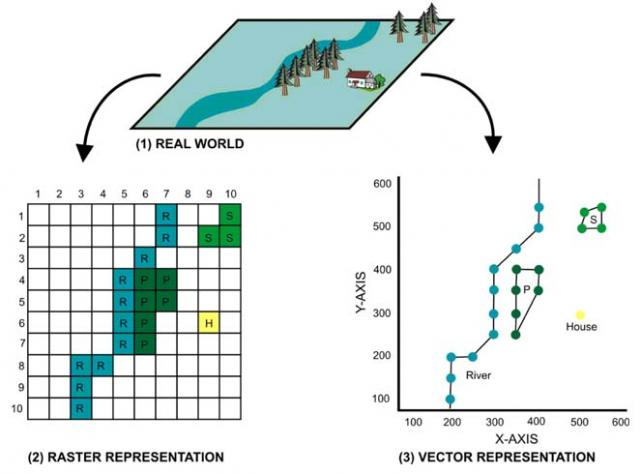
\includegraphics[width=0.8\textwidth]{pics/RasterVectorPreview}
\caption{Realization of raster and vector data representation}
\label{pic:RasterVector}
\end{figure}

Both representations carry various set of advantages and disadvantages. These will be described in the following subsections.

% http://data.geocomm.com/helpdesk/formats.html
\subsection{Raster representation}
Raster type formats consist of equally sized cells arranged in rows and columns to construct the representation of space. Individual cells contain an attribute value and location coordinates. Together they create images of points, lines, areas, networks or surfaces.

\paragraph*{Advantages}
\begin{itemize}[noitemsep]
\item Easy and "cheap" to render
\item Represent well both, discrete (urban areas, soil types) and continuous data (elevation)
\item Grid natures provide suitability for mathematical modeling or quantitative analysis
\end{itemize}

\paragraph*{Disadvantages}
\begin{itemize}[noitemsep]
\item Large amount of data
\item Scaling required between layers
\item Possible information loss due to generalization (static cell size)
\item Difficult to establish network linkage
\end{itemize}

\subsection{Vector representation}
Vector type formats uses vertices as a basic unit. A vertex consists of x and y coordinates to determine its position. Using vertices, it is possible to create any shape to describe any object. One vertex creates a point, two can create a line etc. Objects created by vertices may contain additional attributes about the feature they represent.

\paragraph*{Advantages}
\begin{itemize}[noitemsep]
\item Topology nature
\item Compact data structure
\item Easy to maintain
\item Bigger analysis capability
\end{itemize}

\paragraph*{Disadvantages}
\begin{itemize}[noitemsep]
\item For effective analysis, static topology needs to be created
\item Every update requires rebuilding of topology
\item Continuous data is not effectively represented
\end{itemize}

%\section{Summary -- data usage}
%Most of the official European sources (EuroGeographics, EPSON) require filling a form for each download of data. This process could be the bottleneck for the maintenance efforts of the application, because updating the data would take significant amount of time and would require additional functionality. 

%Next very significant part of the choice is the data format. As was said in subsection HERE_ADD_SECTION well 

\section{Storage}
%TODO
Since the data source and format question is resolved, the next step is to decide the representation of the graph in the memory. During the history of graph theory, three main representations are to choose from. In the following subsections a closer look on all three options will be taken.

\subsection{Adjacency list}
An adjacency list stores a graph as a list of vertices. Each vertex, then, contains an information about its adjacent vertices in form of a linked list. Adjacency list is easy to implement and use. All vertices in a graph are mapped onto the array of pointers referencing to a first node of a linked list. In case, a vertex does not have the adjacent vertices, its pointer is set to null. The example of an adjacency list for a simple graph can be found in Figure \ref{pic:AdjacencyList} and will be further used as example to also explain further representations. 

\begin{figure}[h]
\centering
\includegraphics[width=0.8\textwidth]{pics/GraphRep}
\caption{Representation of a graph using the method of an adjacency list}
\label{pic:AdjacencyList}
\end{figure}


\subsection{Adjacency matrix}
\label{subsec:AdjMatrix}
An adjacency matrix is defined as matrix of a size $|V(G)| \times |V(G)|$, where $V(G)$ is a set of all vertices in graph $ G $. Values within the matrix depend on the type of graph. Generally, adjacency matrix for unweighted graph is defined as a $\textbf{A}(G)=[a_{ij}] $, where $a_{ij}$ is the number of edges joining $v_i$ and $v_j$. If the graph is weighted, the values are from the interval $\langle 0, \infty ) $, where $0$ means two vertices are not adjacent and any non-zero value means they are adjacent with an edge cost of that value\cite{Bondy76}. Although, 1 edge at most must exist between every two vertices.
For the graph G in the example used in Figure \ref{pic:AdjacencyList}, the adjacency matrix $\textbf{A}$ looks like the following:
\[
\textbf{A}(G) =
\kbordermatrix{
 & v_{0} & v_{1} & v_{2} & v_{3} & v_{4} \\
v_{0} & 0 & 1 & 0 & 0 & 1 \\
v_{1} & 0 & 0 & 1 & 1 & 0 \\
v_{2} & 0 & 0 & 0 & 1 & 0 \\
v_{3} & 0 & 0 & 0 & 0 & 0 \\
v_{4} & 0 & 0 & 0 & 1 & 0 	
}
\]
Rows and columns represent vertices of a graph. In the case of matrix $\textbf{A}$, first row and first column represent vertex $0$, second row and column represent vertex $1$ etc. The value in the third row and fourth column means that vertex 2 is adjacent with vertex 3. % As an interesting observation 
It is noticeable that the graph in example $\textbf{A}$ is directed, therefore adjacency matrix is not symmetric. %TODO possible extent of directed/undirected graphs

\subsection{Incidence matrix}
Incidence matrix is very similar to adjacency matrix, but instead of showing relations between vertices themselves it represents relation between vertices and edges. Which means, the size of an incidence matrix is $|V(G)| \times |E(G)|$, whereas $V(G)$ is a set of all vertices and $E(G)$ is a set of all edges in graph $ G $. The incidence matrix of graph G is then $\textbf{M}(G) = [m_{ij}]$, where $m_{ij}$ is the number of times (0, 1 or 2 in case of loop) that the vertex $v_i$ and edge $e_j$ are incident\cite{Bondy76}.

An interesting case is the incidence matrix for a directed graph. In that case the sign of the value within matrix $\textbf{M}$ describes the orientation of the edge. Given the edge $e = (x, y)$, then, in the row of vertex $x$ and the corresponding column for edge $e$, the value is positive. In the row of vertex $y$ and the corresponding column for edge $e$, the value is negative.
For the graph G in the example used in Figure \ref{pic:AdjacencyList}, the incidence matrix $\textbf{M}$ looks like the following:

\[
\textbf{M}(G) =
\kbordermatrix{
 & e_{0} & e_{1} & e_{2} & e_{3} & e_{4} & e_5 \\
v_{0} & 1  & 0  & 1  & 0  & 0  & 0 \\
v_{1} & -1 & 1  & 0  & 1  & 0  & 0 \\
v_{2} & 0  & -1 & 0  & 0  & 1  & 0 \\
v_{3} & 0  & 0  & 0  & -1  & -1  & -1 \\
v_{4} & 0  & 0  & -1 & 0  & 0  & 1
}
\]



\subsection{Sparse matrix}
In mathematics matrices can be divided into two groups: sparse matrices and dense matrices. The definition might sound somehow vague, but sparse matrices are matrices containing huge amount of zero elements. A dense matrix is the exact opposite: containing very few zero elements. In previous subsections it is noticeable that each of the matrices (adjacency and incidence) consist of a lot of zero elements and only a few values are actually useful.

The amount of non-zero elements in the adjacency or incidence matrix depends purely on the degree of vertices in the graph. In both types of matrices, each row serves as a vertex and within non-zero values represent edges incident to the vertex. Depending on the graph is directed or undirected, the amount of non-zero elements in adjacency matrices will differ. Incidence matrices do not change their numbers, because they differ only in sign of the value. 

For undirected graphs, the number of non-zero elements equals to $$ \sum_{v \in V} \textrm{deg(v)} = 2|E| $$ where $E$ is the set of all edges and $V$ the set of all vertices in graph. The same principle applies to the directed graph of incidence matrices. For directed graphs of adjacency matrices, we can observe that the number of non-zero elements depend on amount of outgoing edges $\Rightarrow$ out-degree, which is 
$$ \sum_{v \in V} \textrm{deg\textsuperscript{--}(v)} = |E| $$ where $E$ is the set of all edges, $V$ is the set of all vertices in a graph and $deg\textsuperscript{--}(v)$ function returns number of outgoing edges from the vertex $v$.

The reason for mentioning sparse matrices in the first place is that there are functions and operations which could be done only with the sparse matrices, providing better memory usage. The main motivation for this section are the storage schemes in which sparse matrix could be stored. The usage of storage schemes enable all the advantages of the regular matrix representation with significantly less memory usage since only the non-zero elements are being stored. According to Yousef Saad \cite{Saad03}, main 3 storage schemes will be discussed. 

The coordinate format belongs to the simplest storage schemes of sparse matrices. The data structure consists of three arrays: 
\begin{itemize}
\item an array containing all the (real or complex) values of the non-zero elements of the original matrix in any order
\item an integer array containing their row indices 
\item an integer array containing their column indices
\end{itemize}
All three arrays are of length $N$, which is the number of non-zero elements.

Taking a closer look at adjacency $\textbf{A}$ matrix from section \ref{subsec:AdjMatrix}. Clearly this matrix contains less non-zero elements, therefore it is an example of sparse matrix. Using coordinate format, matrix $\textbf{A}$ looks the following:

$$
\begin{array}{c}

AA:
\begin{array}{|c|c|c|c|c|c|}
 \hline
 1 & 1 & 1 & 1 & 1 & 1 \\
 \hline
\end{array}
\\ \\
IR:
\begin{array}{|c|c|c|c|c|c|}
 \hline
 0 & 1 & 2 & 0 & 1 & 4 \\
 \hline
\end{array}
\\ \\
IC:
\begin{array}{|c|c|c|c|c|c|}
 \hline
 4 & 2 & 3 & 1 & 3 & 3 \\
 \hline
\end{array}
\end{array}
$$

Array $AA$ stores values of non-zero elements, array $IR$ stores the row index of the corresponding element and array $IC$ stores the column index of the corresponding element. The memory needed for storing the matrix is now only $3N$ instead of the original $N^2$.  The coordinate format excels with it's simplicity and flexibility.

If the elements inside array $AA$ are listed by row, the array $IR$ could be transformed to store instead only indices of the beginning of each row. The size of newly defined array $IR$ is then $n+1$, where $n$ is the number of rows in the original matrix. On the last position ($+1$), the number of non-zero elements within the original matrix is being written. It also may be represented as an address, where fictional row begins on $n+1$ position. 

Array $\textbf{A}$, then, would be by this scheme described as the following:

$$
\begin{array}{c}
AA:
\begin{array}{|c|c|c|c|c|c|}
 \hline
 1 & 1 & 1 & 1 & 1 & 1 \\
 \hline
\end{array}
\\ \\
IR:
\begin{array}{|c|c|c|c|c|c|}
 \hline
 0 & 2 & 4 & 5 & 5 & 6 \\
 \hline
\end{array}
\\ \\
IC:
\begin{array}{|c|c|c|c|c|c|}
 \hline
 1 & 4 & 2 & 3 & 3 & 3 \\
 \hline
\end{array}
\end{array}
$$



The transformation of the $IR$ array and listing elements inside $AA$ by row is called Compressed Sparse Row (CSR) format. In scientific computing CSR format is most commonly used for vector-matrix multiplication while having low memory usage.
Through the years, Compressed Sparse Row format developed to a number of variations. 
For example storing columns instead of rows, a new scheme known as Compressed Sparse Column (CSC) format was created.

The last scheme, I would like to point out, is called the Ellpack-Itpack format, which is very popular on vector machines. The Ellpack-Itpack format stores matrices in two 2-dimensional arrays of the same size $n \times N_{mpr}$, where $n$ is the number of rows of the original matrix and $N_{mpr}$ represents the maximum of non-zero elements per row. The first array contains non-zero elements of the original matrix. If the number of non-zero elements is less then the $N_{mpr}$, the rest of the row is filled with zeros. The second array stores the information about the column in which the specific non-zero element is located. For each zero in the first array, any number can be added.

For the given matrix $\textbf{EIF}$:

$$
\begin{array}{c}
\textbf{EIF} = 
\begin{pmatrix}
4 & 0 & 0 & 1 & 0 \\
0 & 0 & 7 & 0 & 9 \\
0 & 2 & 0 & 0 & 0 \\
6 & 0 & 0 & 1 & 0 \\
0 & 0 & 0 & 4 & 3\\
\end{pmatrix}
\end{array}
$$

the Ellpack-Itpack format looks as followed:
 
$$
\begin{array}{lr}
\textbf{AA} = 
\begin{pmatrix}
4 & 1 \\
7 & 9 \\
2 & 0 \\
6 & 1 \\
4 & 3 \\
\end{pmatrix}
\quad \quad
\textbf{IC} = 
\begin{pmatrix}
0 & 3  \\
2 & 4 \\
1 & 0 \\
0 & 3\\
3 & 4 \\
\end{pmatrix}
\end{array}
$$

\subsection{List and matrix comparison}
%Both matrices and list stores equivalent information about the graph. From incidence matrix we can read which two edges share the same vertex (they are incident) and from adjacency matrix which two vertex are connected with an edge. Adjacency list stores for each vertex node edge information in form of linked list which brings two main benefits. 

Adjacency lists in their essence compactly represent existing edges. 
However, this comes at the cost of possible slow lookups of specific edges.
In case of unordered list, the worst case of a lookup time for a specific edge can become O(n), since each list has length equal to the degree of a vertex.
On the other hand, looking up the neighbours of a vertex becomes trivial, and for a sparse or small graph the cost of iterating through the adjacency lists might be negligible.

Adjacency matrices can use more space in order to provide constant lookup times. Since every possible entry exists, it is possible to check for the existence of an edge in constant time using indexes. However, the lookup time for a neighbour becomes O(n) since it is needed to check all possible neighbours.

Data used in the application produce sparse and/or large graphs, for which adjacency list representations suit better.



\section{Preprocessing}

Data are being read from Shapefile source obtained via OpenStreetMaps. After further analysis of the Shapefile provided by Mapzen (Section \ref{subsec:DA_OSM}), each data entry is being represented as a line $\Rightarrow$ two nodes sharing an edge. At this point, the edge is missing its weight. Therefore, first step of preprocessing is to weight all the edges within the graph.

\subsection{Great Circle Distance and Harvesine formulae}
The weight of the edge should represent the price of getting from one node into the other. Our application is trying to find shortest path from multiple sources into one source, therefore the price should be based on the distance between source points and the final node, the shorter the better. 

Each node has its specific coordinates $\Rightarrow$ latitude and longitude. This pair represents unique identifier for every node in the application. Let us have two nodes: node $n$ having coordinates $lat1$ and $long1$, and node $m$ having coordinates $lat2$ and $long2$. If $lat1$ = $lat2 \wedge long1 = long2$, then node $n = m$. If $n \neq m$, then at least one of the coordinates differs between nodes $n$ and $m$ meaning distance between these two nodes is greater than zero.

The simplest solution to compute distance between two points is using the Pythagorean theorem.

$$
d = \sqrt{(\Delta x)^2 + (\Delta y)^2} = \sqrt{(x_2 - x_1 )^2 + (y_2 - y_1)^2}
$$

where $d$ is a distance between the nodes $(x_1, y_1)$ and $(x_2, y_2)$. If we map latitude on $x$-coordinate and longitude on $y$-coordinate, we would get distance between two real points, but in a two dimensional space. For computing the distance on the Earth it is needed to use great circle distance.

The great circle distance takes into account the curvature of the sphere, to provide more precise distance.

To compute the great circle distance on a sphere, harvesine formula is used: 

$$
\begin{array}{l l}
Harvesine formula: & a = \sin^2(\Delta \psi /2) + \cos \psi_1 \cdot \cos \psi_2 \cdot \sin^2(\Delta \lambda /2) \\
& c = 2 \cdot \atantwo ( \sqrt{a}, \sqrt{1 - a} ) \\
& d = R \cdot c
\end{array}
$$ 


\chapter{Design of the application}
\label{ch:DOTA}

\section{SSSP algorithms}
For solving shortest path problems exist nowadays many algorithms. Most of them evolved from their predecessors. Each of them solves the problem with different parameters. 
The following list contains the essential algorithms solving the shortest path problem, which lay the foundation in graph theory science:
\begin{itemize}
\item Dijkstra's algorithm
\item Bellman-Ford algorithm
\item Floyd-Warshall algorithm
\item Johnson's algorithm 
\end{itemize}

The Dijkstra's algorithm \cite{Dijkstra59} and the Bellman-Ford algorithm \cite{Bellman58, FordFulkerson62} solve the single-source shortest path (SSSP) problem. SSSP problem can be defined as: Find the cost of the least cost path from $v$ to $\forall w \in V$, given a directed graph $G = (V,E)$ with non-negative costs on each edge and a selected source node $v \in V$. The cost of a path is simply the sum of the costs on the edges traversed by the path. Dijkstra's algorithm is a greedy algorithm working with the graph were negative edges are not allowed. The Bellman-Ford algorithm is a non-greedy version of the Dijkstra's algorithm which allows to work with graphs having negative edges.

The Floyd-Warshall algorithm \cite{Warshall62, Floyd56} and Johnson's algorithm \cite{Johnson77} solve the all-pair shortest path (APSP) problem. The Floyd-Warshall algorithm iterates all vertices $v$, in order to find a better path for every pair going through $v$ in time $O(N^3)$. Johnson's algorithm, first, converts all the negative edges into positive ones and then, applies Dijsktra's algorithm on every node within the graph. 
For sparse graphs, Johnson's algorithm provides faster computation time than Floyd-Warshall algorithm \cite{Cormen01}.


\section{Dijkstra algorithm}
\label{sec:dijsktra}
The algorithm was conceived by Edsger Wybe Dijkstra in 1956 and was officially published in 1959. Dijkstra's original idea was to find the shortest path between two nodes, however the course of time, among computer scientists, Dijkstra algorithm was accepted as an algorithm finding a path from one single node to all other nodes in the graph. 


% about  Mehlhorn, Kurt; Sanders, Peter (2008). Algorithms and Data Structures: The Basic Toolbox (PDF). Springer.
The Dijkstra algorithm was constructed to solve the applied problem: How to get from one point to another using the shortest path possible. % Frana, Phil (August 2010). "An Interview with Edsger W. Dijkstra". Communications of the ACM. 53 (8): 41–47. doi:10.1145/1787234.1787249
The main criteria used to define the shortest path are either time or distance. Both quantities only have positive values. If these criteria are converted into graph theory, all the edges of the graph need to be also positive.
The data available will only include possitive values, which are the nodes in the graph. Furthermore the graph will represent the geographical map. Therefore Dijkstra algorithm will be the choice of the problem solving algorithm. 

 \subsection{Definition}
There are many variations of Dijkstra algorithm. Here is a presented variation, in which nodes can be in three states: $fresh, open $ and $closed$ (Algorithm \ref{algo_dijkstra}). For each node \textbf{n} the function \texttt{dist}(\textbf{n}) represents the distance from the starting node \textbf{s}. For unreachable nodes the value returned by this function will be undefined. Next to the function \texttt{dist}, there is also the function \texttt{prev}(\textbf{n}), which returns the node for the shortest path back to node \textbf{s}.

\begin{algorithm}[H]
\SetKwFunction{Dist}{dist}
\SetKwFunction{Len}{length}
\SetKwFunction{P}{prev}
\SetKwData{Or}{or}
 set the starting node \textbf{s} as \textit{open} and \Dist{\textbf{s}}$ \leftarrow 0$\;
 \For{for each node \textbf{n} different from \textbf{s}}{
  set node \textbf{n} as \textit{fresh}
 }
 \While{$\exists \textbf{u}$ with state open}
 {
  \textbf{u} $\leftarrow$ $open$ node with minimal \Dist{\textbf{u}} \;
  set \textbf{u} state as $closed$	\;
  \ForEach{neighbour \textbf{w} of \textbf{u}}
  {
   \If{\textbf{w} is fresh \Or \Dist{\textbf{w}} $ > $  \Dist{\textbf{u}} $+$ \Len{\textbf{w}, \textbf{u}}}{
	\lIf{\textbf{w} is fresh}{ 
	set \textbf{w} as open}
	\Dist{\textbf{w}} $\leftarrow$ \Dist{\textbf{u}} $+$ \Len{\textbf{w}, \textbf{u}}\;
	\P{\textbf{w}} $\leftarrow \textbf{u}$   
   }
  } 
 }
\caption{Dijkstra algorithm}\label{algo_dijkstra}
\end{algorithm}

On the line number \textbf{6} the choice of the node \textbf{u} means choosing the \textbf{u} with \texttt{dist}(\textbf{u}) $ \leq $ \texttt{dist}(\textbf{w}), where \textbf{w} is every other node having the state $open$.

\subsection{Proof of correctness}

In order to prove the algorithm will stop after finite number of step and its correctness, it is needed to define lemma about states in which nodes can be:

%%%%% LEMMA 1
\begin{lemma}
Nodes can only change state either from "\textit{fresh}" to "\textit{open}" or from "\textit{open}" to "\textit{closed}".
\end{lemma}
%%%%% LEMMA 1

%%%%% PRoof1
\begin{proof}
The only time nodes can change state are on line \textbf{7} and \textbf{10} of the Algorithm \ref{algo_dijkstra}.
\end{proof}
%%%%% PRoof1

%%%%% Theorem 2
\begin{theorem}
\label{theorem2}
Dijkstra algorithm will stop computing after at the most \textit{N} steps iterations of while cycle, where N is a number of nodes in graph. 
\end{theorem}
%%%%% Theorem 2

%%%%% Proof 2
\begin{proof}
From the description of the algorithm and previous lemma it is clear the set of closed nodes of cycle will increase with each iteration by one and its size being between 0 and \textit{N}.
\end{proof}
%%%%% Proof 2

%%%%% Theorem 3
\begin{theorem}
Let $A$ be a set of closed nodes. The length already found path from $v_0$ to $v$ is the length of the shortest path $v_0 v_1 \dots v_k v$, where nodes $v_0, v_1, \dots , v_k$ are in set $A$.
\end{theorem}
%%%%% Theorem 3

%%%%% Proof 3
\begin{proof}
The proof is by induction on the number of step executed. The theorem clearly is correct before and after the first step. 

Let $w$ be a node with a state set to closed in last step. Let us consider a node $v$ which is closed.
If $v=w$, then the theorem is trivial. In opposite case case we will show, that there is a shortest path from $v_0$ to $v$ through nodes in set $A$ not containing the node $w$. Set $L$ as a length of the path from $v_0$ to $v$ through the nodes in $A$ without $w$. Because in each step we choose node with the lowest \texttt{dist}(\textbf{u}) and \texttt{dist} of chosen nodes in each step represents nondecreasing sequence (weight of the edges are positive), then the length of the path from $v_0$ to $w$ through nodes in $A$ is at least $D$. Because we have chosen the $D$ we know, there exists a path from $v_0$ to $v$ through nodes in $A$ which is not using node $w$.

Now let us consider a node $v$ which is not closed. Let $v_0 v_1 \dots v_k v$ be the shortest path from $v_0$ to $v$, where $\forall v_0, v_1, \dots v_k v \in A$. 
If $v_k = w$, then we changed the \texttt{dist} to the length of this path in current step. If $v_k \neq w$ then $v_0 v_1 \dots v_k$ is the shortest path from $v_0$ to $v_k$ through nodes in $A$ and so we can assume that no nodes $v_0, v_1, \dots v_k $ is not $w$ (according to last paragraph). Hence the length of the path was already set to the correct value before current step.

Due to the fact, that after last step the set $A$ contains only the nodes, into which exists a path from node $v_0$, we have proven the correctness of Dijkstra algorithm.
\end{proof}
%%%%% Proof 3

\subsection{Time complexity}
Now from the Algorithm \ref{algo_dijkstra} we can compute time general complexity of Dijkstra algorithm. Let us assume we use array in order to store the distances for all the $N$ nodes. As proven in Theorem \ref{theorem2} the whole algorithm will execute at most $N$ steps, in each we are choosing node from the set of \textit{fresh} nodes having size $O(N)$. In each step we also need to check the number of nodes, which are being connected via edges outgoing from the currently checked node. Number of these checks in total is equal to at most $O(E)$, where $E$ is a number of edges in the input graph. To sum up time complexity equals to $O(N^2 + M)$, i.e. $O(N^2)$ since $E$ can be at the most $N^2$.

It is possible to improve this complexity by using heap instead of an array in order to store the distances. In the beginning the heap will contain $N$ elements and in each step this number will be reduced by one: We find and delete smallest one in a time of $O(\log{N})$ and adjusting the distances of the neighbours, which takes $O(E\log{n})$ through all the edges. In total the time complexity of the algorithm is $O((N+M) \log{N})$. As mentioned in Section \ref{sec:dijsktra} for real life problems we expect the graph having a form of a sparse graph, meaning for $M << N^2$ the heap version of the algorithm will provide much more better results.


Dijkstra algorithm is very similar to Bellman-Ford algorithm mentioned in subsection \ref{sec:SPP}. The main difference between these algorithms is repetitive checking of the nodes. Once Dijkstra algorithm closes a node, it will never be checked again. Bellman-Fold algorithm goes through each of the nodes and recalculates the path in case negative edges exists in the graph. Because of this extra step, it is slower then Dijkstra, but can detect whether the graph is valid or not.

Dijkstra algorithm computes shortest paths from one single node to all of the others in the graph. However, the Meeting Scheduler application is searching optimal point given multiple input locations instead of single one. After applying Dijkstra algorithm on every input node, the graph instance now contains shortest paths for each input node. Therefore, every node in the graph holds an information about the distance to each of the input nodes. Within these nodes exists one node, having the optimal combination of shortest paths, which is the result the Meeting Scheduler application.
This whole computation process leaves a lot of space for the performance optimization, especially parallelization. 

\section{Parallelization of Dijkstra algorithm}
As mentioned in previous section, the Meeting Scheduler application applies Dijkstra algorithm on each of the input nodes. As a result every node stores the information about the shortest path to each of the input nodes. 

\section{User interface design}
The application requires the spacial information as the input. 
Further, the user should be able to insert the positions of people in order to find a meeting, which is approximately of the same distance to all positions. For that, the user interface (UI) of the application should provide a way to register and store spacial information provided by the user. 

Creating a fully satisfiable graphical user interface (GUI) is not main purpose of this thesis, so it was decided to create a simple GUI in which users can insert the geographical coordinates of participants. As a result, a single pair of coordinates of final destination will be received. 

A fully optimal GUI would allow users to select a position through the displayed map of the dataset available. That way finding exact coordinates would be further transcribed into a marked point on the map and the general user-flow would be significantly improved, because the user would see a marked point on the map which would be the meeting point. 

\chapter{Realisation}
\label{ch:Realisation}

\section{Frameworks used}
The goal of the thesis is to create complex desktop application with basic front-end to provide user proper control over the input data and general overview over the application. In addition, the technology used should be cross-platform. In general, modern high-level programming languages prefer one platform over the other (C\texttt{\#} Windows, ObjC iOS etc.). 

In direction of keeping the application as simple as possible, the main computation part of the application is written in C\texttt{++} language, which provides great computing performances on any platform while offering OOP principles in order to create more complex applications. In addition, C\texttt{++} based back-end will make deployment on any server operating system effortless. Not to mention there are plenty open source libraries available making a realization of the whole project easily done.  

%% QT 
One of the external tools used for the purpose of the application is Qt framework. Qt provides cross-platform tools to create basic GUI and is classified as FOSS computer software, therefore fitting the purpose of the application being open source. 
Usage of classes and functions of Qt framework is very straightforward while producing fully functional GUI as a front end for the application. 

%% GDAL
For reading the data files and following manipulation GDAL/ORG library was selected. GDAL is designed to read and write raster GIS formats. GDAL library is developed under Open Source Geospatial Foundation and released under the X/MIT license. 
As an addition to the GDAL is the ORG library which enables usage of simple features for vector formats. Together the whole GDAL/ORG library supports most of the GIS formats. %cite "GDAL Raster Formats". GDAL - Geospatial Data Abstraction Library. 2011-06-05.	
Since the dataset of the application is in Shapefile format, GDAL/ORG library provides optimal tools for reading and collecting information from our dataset.

\section{Server}



\subsection{Data processing part}

\subsubsection{Data}
%TODO FITNESS, STORAGE, Source


\subsection{Computation part}

\subsubsection{Algorithm}

\subsubsection{Parallelization}

\section{Client}


\chapter{Results}
\label{ch:Results}

\section{Speed}

\section{Preciseness}

\setsecnumdepth{part}
\chapter{Conclusion}

\bibliographystyle{iso690}
\bibliography{mybibliographyfile}

\setsecnumdepth{all}
\appendix

\chapter{Acronyms}
% \printglossaries
\begin{description}
	\item[APSP] All-pair shortest path
	\item[CERCO] Comit{\' e}e Europ{\' e}en des Responsables de la Cartographie Officielle\item[GUI] Graphical user interface
	\item[DEM] Digital Elevation Model
	\item[ERDF] European Regional Development Fund
	\item[ESPON] European Observation Network for Territorial Development and Cohesion
	\item[FOSS] Free and Open-Source Software
	\item[GDAL] Geospatial Data Abstraction Library
	\item[GIS] Geographic information systems	
	\item[MEGRIN] Multi-purpose European Ground Related Information Network
	\item[OOP] Object Oriented Programming
	\item[OSM] OpenStreetMaps
	\item[SSSP] Single-source shortest path
	\item[XML] Extensible markup language
	
	
\end{description}


\chapter{Contents of enclosed CD}

%change appropriately

\begin{figure}
	\dirtree{%
		.1 readme.txt\DTcomment{the file with CD contents description}.
		.1 exe\DTcomment{the directory with executables}.
		.1 src\DTcomment{the directory of source codes}.
		.2 wbdcm\DTcomment{implementation sources}.
		.2 thesis\DTcomment{the directory of \LaTeX{} source codes of the thesis}.
		.1 text\DTcomment{the thesis text directory}.
		.2 thesis.pdf\DTcomment{the thesis text in PDF format}.
		.2 thesis.ps\DTcomment{the thesis text in PS format}.
	}
\end{figure}

\end{document}
